% time values for run8 and run9
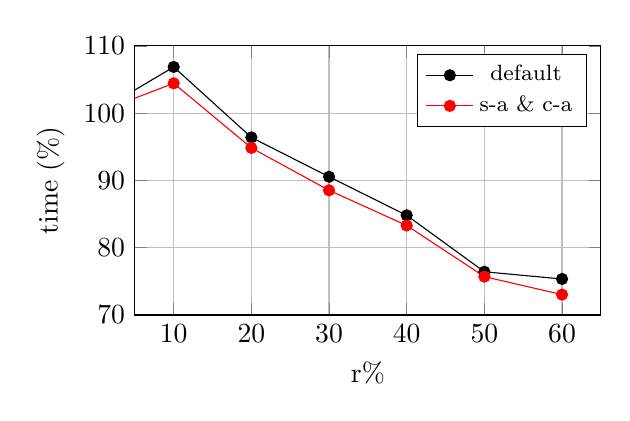
\begin{tikzpicture}
\begin{axis}[
    title={},
    height=5cm,
    width=7.5cm,
    xlabel={r\%},
    ylabel={time (\%)},
    xmin=5, xmax=65,
    ymin=70, ymax=110,
    xtick={0,10,20,30,40,50,60},
    ytick={70,80,90,100,110},
    legend pos=north east,
    xmajorgrids=true,
    ymajorgrids=true,
    legend style={font=\footnotesize}
]

\addplot[
    color=black,
    mark=*
    ]
    coordinates {
    (0,100)(10,106.86)(20,96.39)(30,90.54)(40,84.81)(50,76.42)(60,75.35)
    };
    
\addplot[
    color=red,
    mark=*
    ]
    coordinates {
    (0,100)(10,104.43)(20,94.83)(30,88.53)(40,83.30)(50,75.70)(60,73.03)
    };
    
\legend{default, s-a \& c-a}
    
\end{axis}
\end{tikzpicture}